\section{摘要}
\begin{frame}{摘要}
    在现实世界中,有许多金融企业在运营中爆发危机的案例,例如1998年LTCM公司遭遇俄债违约导致巨额亏损、2008年雷曼兄弟破产。许多情况下人们将金融危机的爆发归结于企业风险管理的失败,但是\citeauthor{stulz2008risk}的这篇文章\citetitle{stulz2008risk}认为金融危机的爆发并不能说明企业的风险管理失败。
\end{frame}

\section{文献背景}
\begin{frame}{LTCM简介}
    美国长期资本管理公司(Long-Term Capital Management,LTCM)是 1994 年在美国创立的一家对冲基金公司。这家公司有两位著名成员迈伦·斯克尔斯(Myron Scholes)和罗伯特·默顿(Robert Merton)。
    LTCM自创立以来,一直保持骄人的业绩,在华尔街乃至全世界一路高歌。这个汇聚了职业巨星、公关巨星、学术巨星的精英团队在创立之后的 4 年里取得了辉煌的业绩,收益报酬率年化高达20\%,很多大型银行和富豪们争先恐后地把资金委托给LTCM管理。
    \begin{figure}
        \centering
        \begin{minipage}{0.48\linewidth}
            \centering
            
\includegraphics[width=0.4\linewidth]{img/Merton.jpg}
        \end{minipage}
        \begin{minipage}{0.48\linewidth}
            \centering
            
\includegraphics[width=0.4\linewidth]{img/Scholes.png}
        \end{minipage}
        \caption{Merton(左)与Scholes(右)因期权定价理论获1997年诺贝尔经济学奖}
    \end{figure}
\end{frame}

\begin{frame}{LTCM交易策略}
    LTCM采取了配对套利交易策略,利用性质相似的两个资产之间存在一定价格关系而进行的方向相反的交易活动,其交易标的包括全球各国的政府国债、公司债券以及房屋抵押证券等。
    \begin{enumerate}
        \item 通过数学模型计算出利差,预期两种债券间的利差将会缩小;
        \item 融券价格被高估的债券并卖出,然后买入价格被低估的债券;
        \item 当未来两者的利差缩小时,多头空头同时获利。
    \end{enumerate}
    \begin{figure}
        \centering
        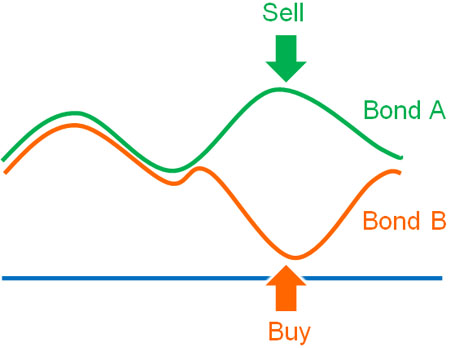
\includegraphics[width=0.5\linewidth]{img/ltcm.jpg}
    \end{figure}
\end{frame}

\begin{frame}{巨额的收益回报}
    为了进一步扩大收益,LTCM还在套利策略的基础上加了高杠杆,通过如此激进的套利交易模式,从1994年4月开始运作到1997年10月,LTCM累计投资回报率高达300\%,公司的资产净值从成立之初的10亿美元上升到47亿美元。
    \begin{table}
        \caption{LTCM回报}
        \begin{tabular}{|c|ccc|}
        \hline
                & 年化收益 & 年化收益(去除管理费) & 投入\$10000剩余 \\\hline
        1994-12 & 28\% & 20\%        & \$12000     \\
        1995-12 & 59\% & 43\%        & \$17160     \\
        1996-12 & 57\% & 41\%        & \$24196     \\
        1997-12 & 25\% & 17\%        & \$28309     \\
        1998-12 & -    & -92\%       & \$2300     \\\hline
        \end{tabular}
    \end{table}
\end{frame}

\begin{frame}{国际政府债券套利}
    在国际债券市场上,公司预期俄罗斯、日本等国家的债券价格被低估,未来这些国家与美国、德国等发达国家的政府债券利差将进一步缩小,因此LTCM持有俄罗斯、日本国债的多头,并利用美国国债的空头来对冲。1998年8月17日,而当天俄罗斯政府突然宣布卢布贬值,并宣布冻结281亿卢布(135亿美元)的国债,停止国债交易。
    \begin{figure}
        \centering
        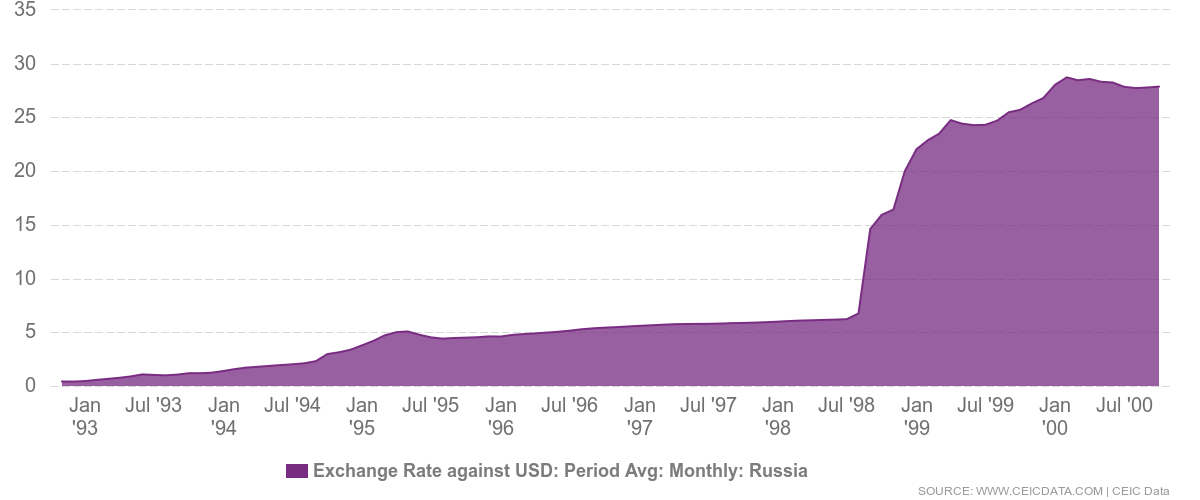
\includegraphics[width=\linewidth]{img/rub_usd.png}
    \end{figure}
\end{frame}

\begin{frame}{承受巨额损失导致破产}
    这一事件迅速发酵,致使投资者纷纷从新兴市场撤出转而投向美国、德国等低风险国债品种,西方国家与新兴市场的债券价差大幅拉开,LTCM遭受暴击。
    \begin{figure}[H]
        \centering
        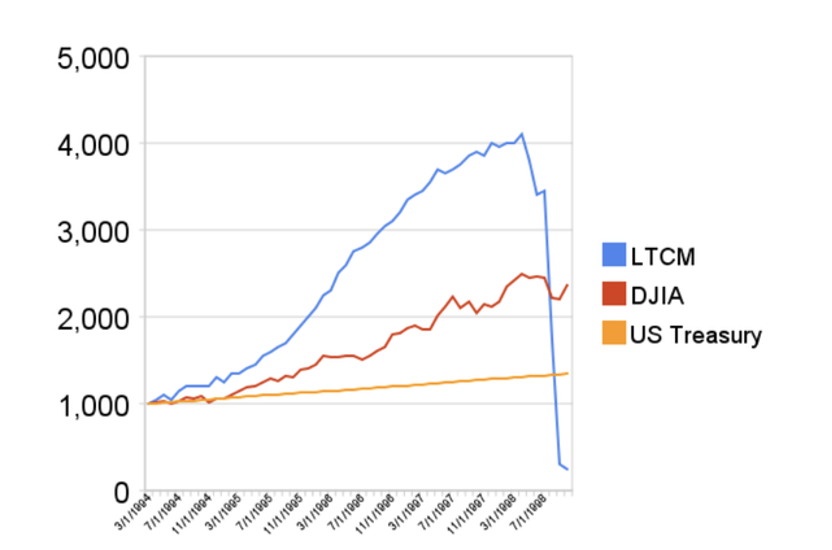
\includegraphics[width=0.8\linewidth]{img/图片 1.png}
        \caption{LTCM基金净值走势与道琼斯指数及美国国债收益率对比}
    \end{figure}
\end{frame}
\begin{frame}{承受巨额损失导致破产}
    到1998年8月底,LTCM的资本就已经降到了23亿美元,失去了年初时超过半数的股权资本。考虑到当时LTCM的资产基数约为1070亿美元,所以公司的杠杆比率已超过45倍。

    由于LTCM对策略和持仓持有非常严格的保密协议,他们会将每个策略分割成不同的交易,分别交给不同的银行执行。这样的做法就使得在风险爆发之时,如果公司合约分属不同的交易对手,那么LTCM需要为每个交易对手都提供高昂的保证金。
\end{frame}
\section{风险管理失败的类型}

\begin{frame}{风险管理失败的类型}
    LTCM破产的案例中,使许多人将如此结果的原因归结于LTCM的风险管理失败,但是在文献中,作者认为LTCM遭遇俄债的可能只是正确管理风险后发生的极低概率损失事件。作者定义了六种风险管理的类型,分别为:
    \begin{itemize}
        \item \nameref{sec:1}
        \item \nameref{sec:2}
        \item \nameref{sec:3}
        \item \nameref{sec:4}
        \item \nameref{sec:5}
        \item \nameref{sec:6}
    \end{itemize}
\end{frame}

\subsection{对已知风险的错误预测}\label{sec:1}

\begin{frame}{对已知风险的错误预测}
    现实中,各家企业的风险管理部门依据数学模型、历史经验以及风险模拟来预测风险发生的概率分布,然后根据企业的风险容忍度做出相应的决策。如果企业对于风险发生的概率进行了错误的判断。

    以LTCM事件为例,公司内部的利差预测模型判断未来俄罗斯国债和美国国债利差将缩小,同时对于俄罗斯国债违约公司内部判断存在这样的风险会导致巨额损失,但是对于如此体量的国家来说出现违约属于极低概率事件,所以LTCM在识别出风险之后依然进行套利操作。

    我们认为, LTCM在对于俄罗斯政府的财务状况以及政府行为了解不充分,过度依赖于数学模型的预测结果。LTCM由于自身在风险预测上的不完备,低估了俄罗斯发生违约的概率,导致风险管理的失败。
\end{frame}

\subsection{忽略未知风险}\label{sec:2}

\begin{frame}{忽略未知风险}

    风险识别时如果遗漏了未知的风险,进行决策时没有考虑到,那么该风险一旦发生将会为企业带来巨大的损失。

    例如2021年的教培行业,许多私募在投资该领域时,从未意识到延续了几十年的教培行业存在被政策叫停的风险。当双减政策出台,许多教培企业被迫关门,投资者遭受巨额的亏损。

    在LTCM的案例中,LTCM内部的风险报告中识别到了存在违约风险,因此从这一点来看,不属于是这一类型的风险管理失败。
    \begin{figure}
        \centering
        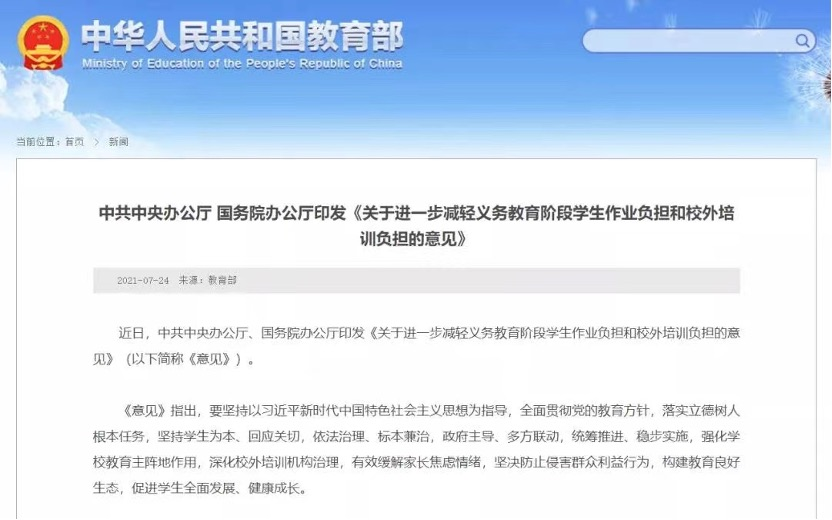
\includegraphics[width=0.4\linewidth]{img/图片 1.jpg}
        \caption{2021年7月双减政策出台}
    \end{figure}

\end{frame}
\subsection{内部沟通失效}\label{sec:3}
\begin{frame}{内部沟通失效}
    风险管理是为了使整个公司股东利益最大化而作出的行为,除了风险管理部门还需要各部门的协调配合,风险管理人员提供相关的风险信息,最终由管理层作出决策,各部门配合执行。但是如果企业内部的沟通失效,将会导致整个风险管理体系的失败。

    内部沟通失败主要有两种情况,第一种是传递的信息出现扭曲,管理层错误理解了风险管理部门输出的信息,进而做出了不合适的决策;第二种是风险管理部门传递信息存在时滞,使风险管理体系失效。LTCM的例子中,我们认为并未出现沟通机制的失效,不存在这一类型的风险管理失败。
\end{frame}
